% TCGA-BRCA. Compile: pdflatex, biber, pdflatex, pdflatex.
% Template sourced from Paul's Notes, a recycled and emptied manuscript template.
% it compiles. 

% README .tex must be compiled through BIBER, to include references! 
% in tex shop select pdflatexmk, from the drop down menu!



% ============================================================
% TeXShop Compilation Guide (macOS)
% ============================================================
% 1. Place the .tex and .bib files in the same directory.
% 2. Open the .tex file in TeXShop.
% 3. Select "pdflatexmk" from the Typeset dropdown.
% 4. Click "Typeset" to compile the manuscript.
% 5. pdflatexmk automatically handles the required LaTeX
%    and Biber passes when properly configured.
%
% Citations: \parencite{reference_key}
% References: \printbibliography[title={References}]
%
% If citations fail, run the following in Terminal:
%   pdflatex manuscript.tex
%   biber manuscript
%   pdflatex manuscript.tex
%   pdflatex manuscript.tex
%
% Replace "manuscript" with the actual filename.
% ============================================================
% !TEX TS-program = pdflatexmk

%End readme.



\documentclass[12pt,letterpaper]{article}
% Image and figure support - we need this to import our images. 
\usepackage{graphicx}
\usepackage{booktabs}
\usepackage{placeins}
\usepackage{float}
\usepackage{caption}
\usepackage{booktabs}
\usepackage[T1]{fontenc}
\usepackage[utf8]{inputenc}
\usepackage{mathptmx}
\usepackage[margin=1in,headheight=15pt]{geometry}
\usepackage{setspace,fancyhdr,titlesec}
\usepackage[american]{babel}
\usepackage{csquotes}
\usepackage[backend=biber,style=apa]{biblatex}
\DeclareLanguageMapping{american}{american-apa}
%this is how we pipe in the bibliography, 
%if you use a staged .bib in git, for professional work, it go much faster then hand type.
%in git hub, place .bib into a list, then call the list. each ref is object -> pipe into call.
\addbibresource{Skeffington_Paul_TCGA_BRCA_References.bib}

% removed [hidelinks]
% We need links for TCGA compliance, to link to their website as per citation guidance. 
% Hyperlink colors: blue for URLs, citations, and internal links
\usepackage{xcolor}
\definecolor{linkblue}{HTML}{0072B2}

\usepackage[
    colorlinks=true,
    linkcolor=linkblue,
    citecolor=linkblue,
    urlcolor=linkblue
]{hyperref}

\captionsetup[table]{
    font=small,
    labelfont=bf,
    justification=raggedright,
    singlelinecheck=false,
    skip=8pt
}

\pagestyle{fancy}\fancyhf{}\fancyhead[R]{\thepage}\renewcommand{\headrulewidth}{0pt}
\doublespacing\raggedright\setlength{\parindent}{0.5in}\setlength{\parskip}{0pt}
\setcounter{secnumdepth}{0}
\titleformat{\section}{\normalfont\normalsize\bfseries\filcenter}{}{0pt}{}
\titlespacing{\section}{0pt}{\baselineskip}{0.5\baselineskip}
\setlength{\bibhang}{0.5in}
\newcommand{\papertitle}{TCGA-BRCA: Gene Expression and PAM50 Visualization}
\begin{document}
% cover page.
\begin{titlepage}
\thispagestyle{fancy}
\vspace*{1.6in}
\begin{center}
\textbf{\papertitle}\\[2\baselineskip]
Paul A. Skeffington\\
Master of Science in Health Data Science\\
Geisel School of Medicine at Dartmouth\\[\baselineskip]
Foundations in Data Science\\
HSE.711-FA26 \textbar{} HDOFA26\\
Instructor: Dr. Shira Fisher\\
Teaching Assistant: Erica Paulos\\[\baselineskip]
\today
\end{center}
\end{titlepage}
\setcounter{page}{2}
\begin{center}\textbf{\papertitle}\end{center}


%peroid goes after \parencite!


\section*{Introduction}

Breast cancer represents a major global public health challenge requiring multinational collaboration in scientific research and pharmaceutical development. In 2024, approximately 2.4 million women were diagnosed with breast cancer worldwide, with an estimated 694,000 associated deaths \parencite{who2026breast}. Despite advances in screening and treatment, breast cancer remains a biologically heterogeneous disease, exhibiting considerable variation in molecular characteristics and clinical behavior.

Through the contributions of scientists worldwide, gene-expression research has identified distinct molecular subtypes, including Luminal A, Luminal B, HER2-enriched, and Basal-like breast cancers \parencite{parker2009}. These classifications demonstrate differences in tumor biology and provide researchers with a framework for investigating variation in gene expression. The Cancer Genome Atlas (TCGA) has established an extensive molecular resource for investigating breast cancer heterogeneity \parencite{tcga2012}.

Two genes, ESR1 and ERBB2, were selected for their associations with estrogen signaling and HER2-related growth pathways, respectively \parencite{tcga2012}. ESR1 (Estrogen Receptor 1) encodes estrogen receptor alpha, which regulates hormone-dependent gene expression and is strongly associated with luminal breast cancer subtypes \parencite{parker2009}. ERBB2 (HER2) encodes a receptor tyrosine kinase involved in cellular growth and survival, with amplification or overexpression associated with HER2-positive breast cancer \parencite{tcga2012}.

% ============================================================
% Methods — IN PROGRESS
% ============================================================

\section*{Methods}

We examined the supplied gene-expression matrix (\texttt{counts.csv}) and associated sample annotations (\texttt{meta\_data.csv}). The results presented here are based, in whole or in part, on data generated by the \href{https://www.cancer.gov/tcga}{TCGA Research Network}.

TCGA was made possible through the voluntary contributions of patients who consented to the use of their biological specimens and associated clinical information for cancer research. These donated tissue samples and accompanying clinical data have enabled significant advances in the genomic and molecular characterization of cancer. TCGA established informed-consent procedures and data-access safeguards to protect participants' rights while supporting scientific research. These patient contributions continue to advance our understanding of breast cancer heterogeneity.

[State the verified data origin and assay, how sample identifiers were matched, the selected sample types, exclusions, and the exact subtype field.]

[Describe any gene filtering, normalization or transformation, Z-score calculations, and how genes were selected for visualization.]

Descriptive statistics and a heatmap were used to characterize the selected cohort. An exploratory volcano plot was generated to illustrate differences between specified sample groups.

[State the actual comparison, calculation of effect sizes and p-values, and any multiple-testing adjustment.]

Unless an appropriate count-based statistical model was fitted, these comparisons should be interpreted as exploratory rather than confirmatory \parencite{love2014,benjamini1995}.


% ============================================================
% RESULTS — IN PROGRESS
% ============================================================
\section*{Results}

[Report the final matched sample count and molecular subtype distribution, including denominators and missing annotations.]

[Report reproducible descriptive findings from the gene-expression summaries.]

[Reference the final heatmap and briefly describe its most relevant expression patterns, noting that Z-score tails do not represent statistical significance.]

[Reference the final volcano plot and identify the comparison groups, axes, thresholds, and methodological limitations. Do not interpret exploratory highlights as validated differential-expression findings.]



% ============================================================
% FIGURES — FIGURES WORKING NO TOUCH
% Figures are stored in figures folder in submission .zip.
% ============================================================
\clearpage
\section*{Figures}


% Figure 1 — PAM50 subtype visualization
\begin{figure}[H]
    \centering
    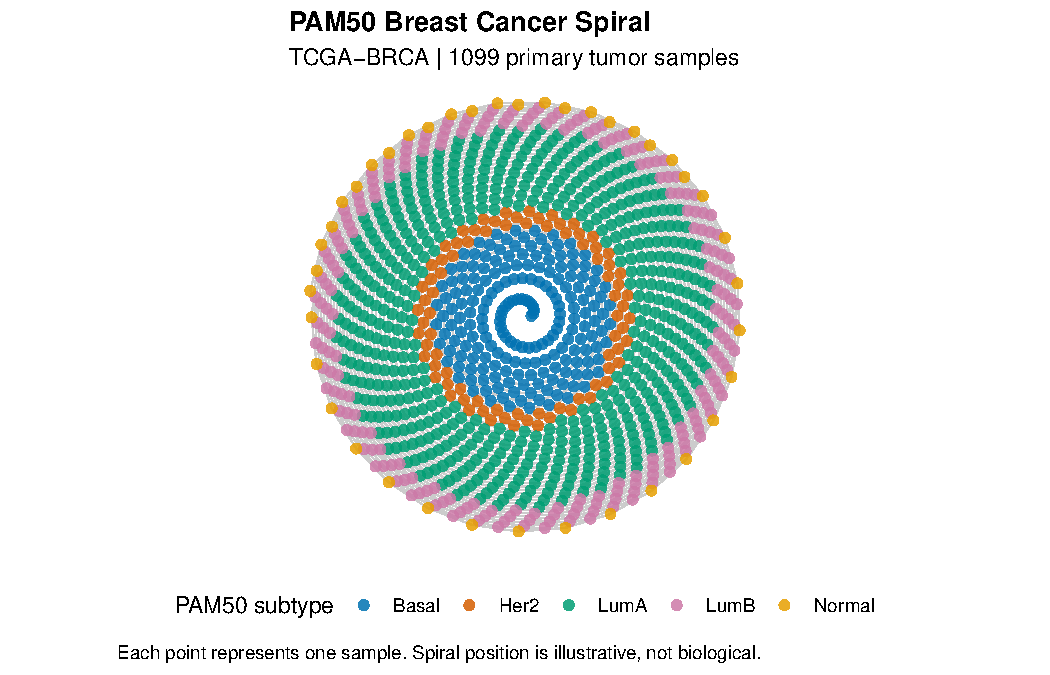
\includegraphics[width=0.85\textwidth]{figures/pam50_spiral.pdf}
    \caption{Visualization of PAM50 molecular subtypes
    in the TCGA-BRCA cohort.}
    \label{fig:pam50}
\end{figure}

% Figure 2 — ESR1 expression distribution
\begin{figure}[H]
    \centering
    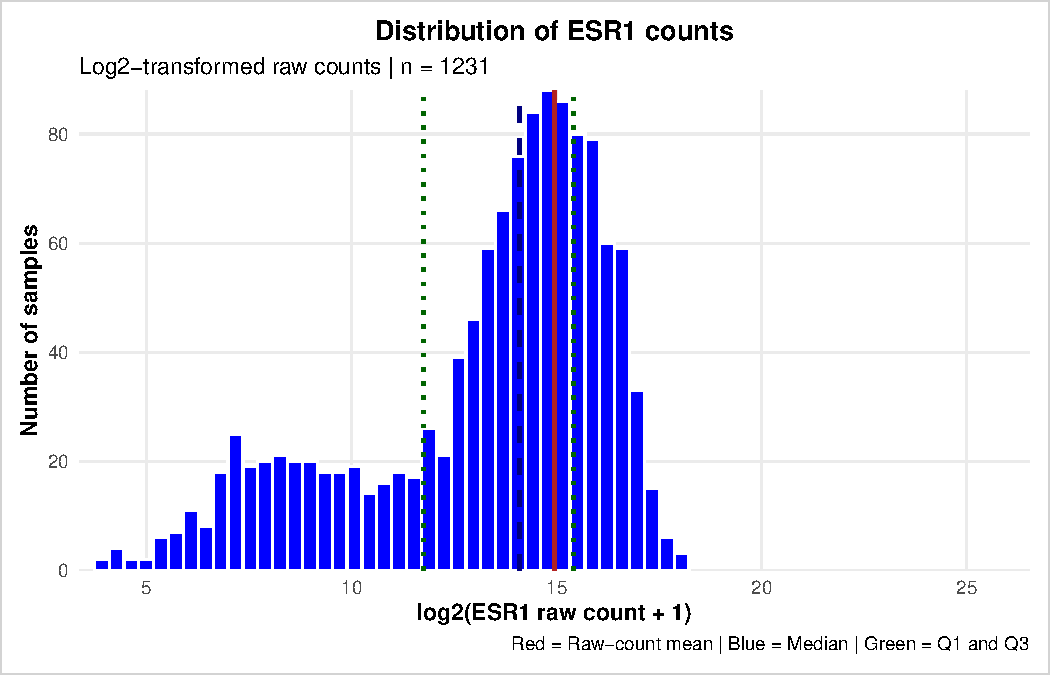
\includegraphics[width=0.85\textwidth]{figures/esr1_histogram.pdf}
    \caption{Distribution of ESR1 gene-expression values.}
    \label{fig:esr1_hist}
\end{figure}

% Figure 3 — ESR1 by sample type
\begin{figure}[H]
    \centering
    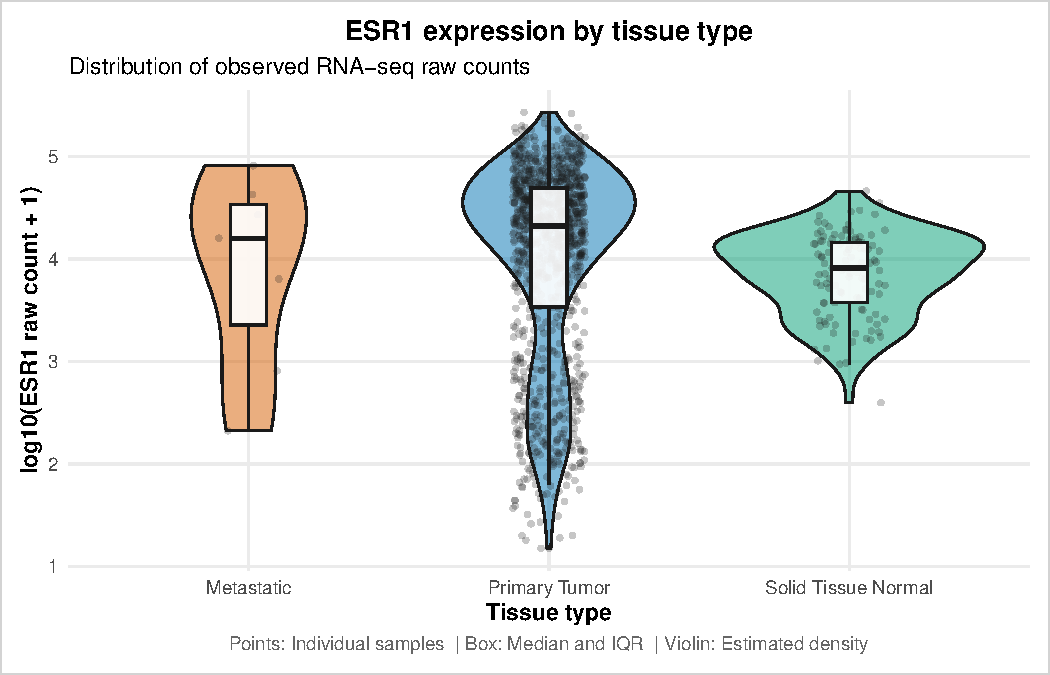
\includegraphics[width=0.85\textwidth]{figures/esr1_sample_type.pdf}
    \caption{ESR1 expression across sample types.}
    \label{fig:esr1_sample}
\end{figure}

% Figure 4 — ESR1 by PAM50 subtype
\begin{figure}[H]
    \centering
    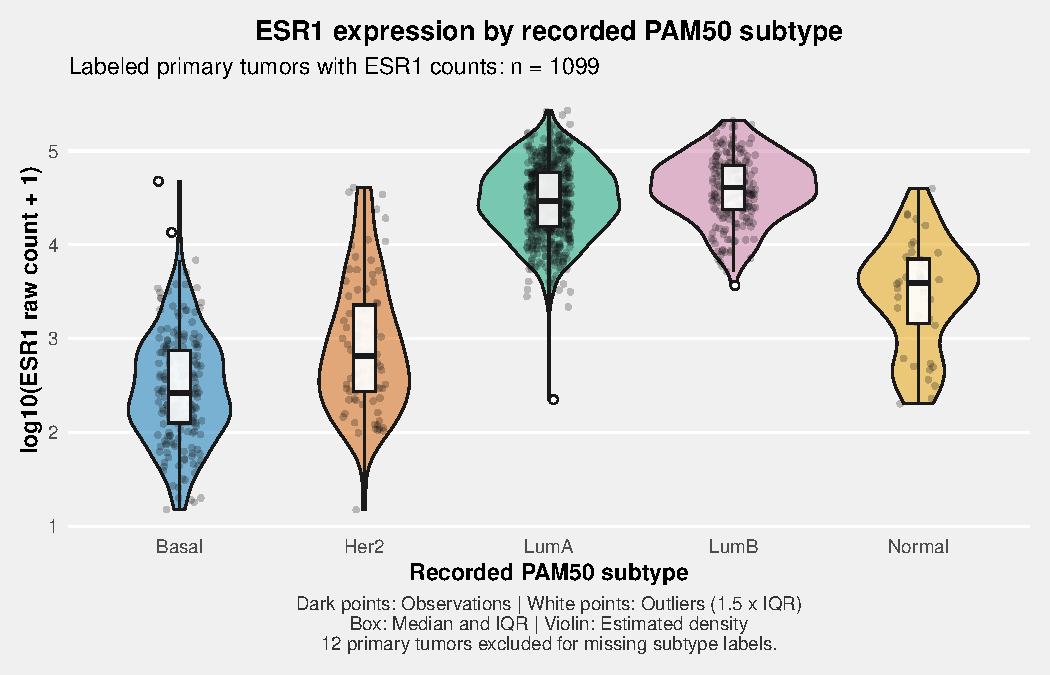
\includegraphics[width=0.85\textwidth]{figures/esr1_subtype.pdf}
    \caption{ESR1 expression across PAM50 molecular subtypes.}
    \label{fig:esr1_subtype}
\end{figure}

% Figure 5 — Gene-expression scatterplot
\begin{figure}[H]
    \centering
    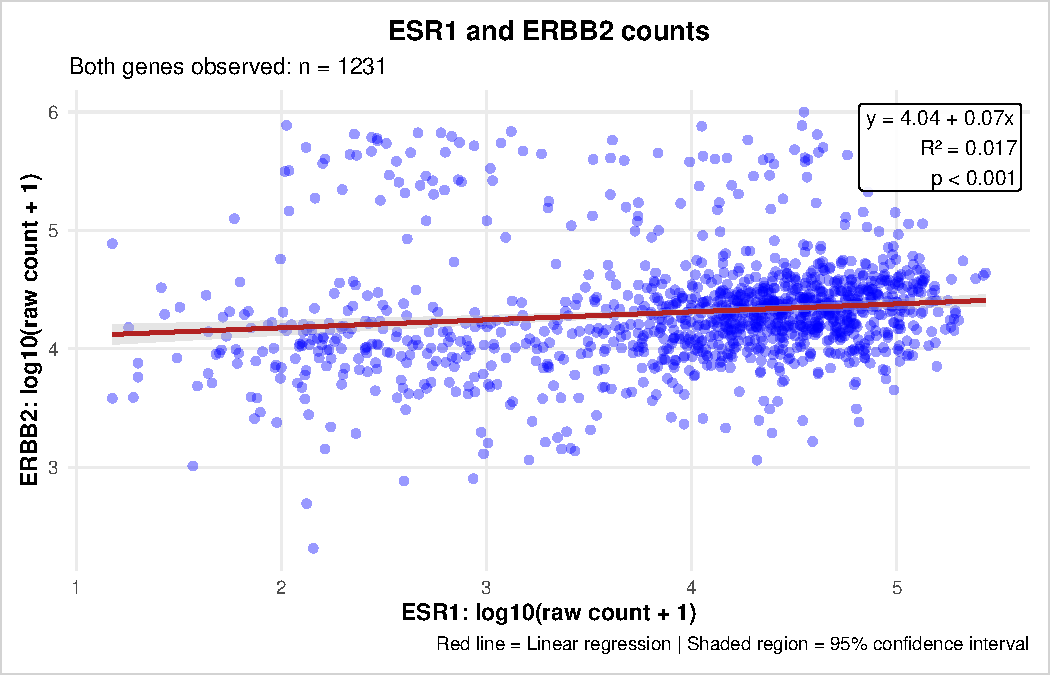
\includegraphics[width=0.85\textwidth]{figures/gene_scatter.pdf}
    \caption{Exploratory gene-expression scatterplot.}
    \label{fig:scatter}
\end{figure}

% Figure 6 — Gene-expression heatmap
\begin{figure}[H]
    \centering
    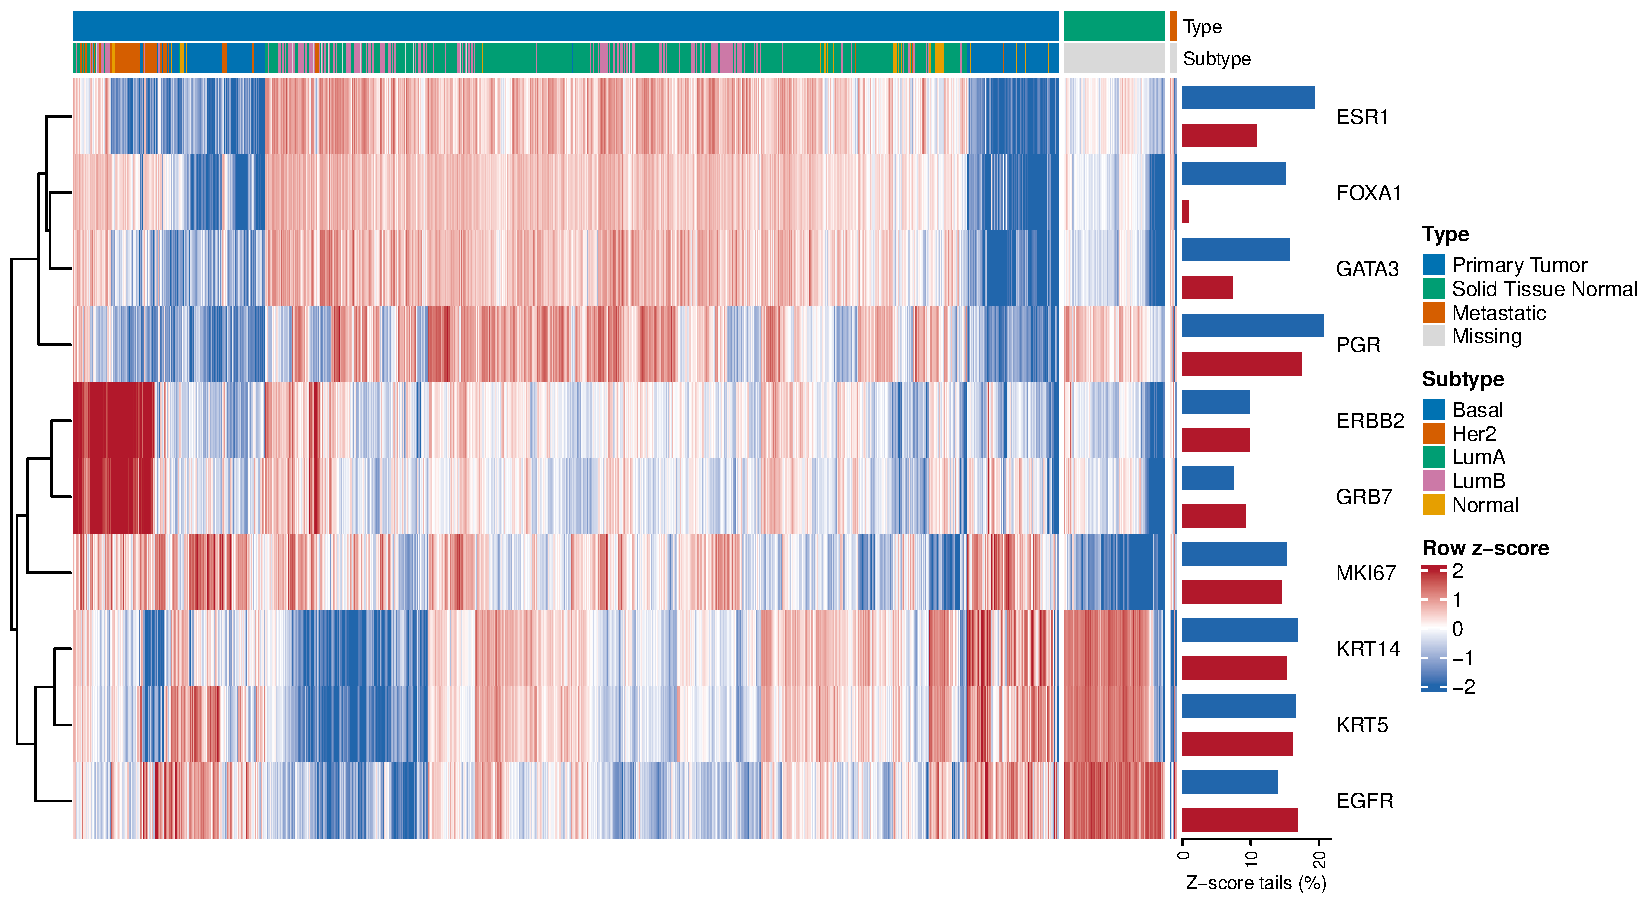
\includegraphics[width=\textwidth]{figures/gene_heatmap.pdf}
    \caption{Heatmap of selected breast cancer-associated
    gene-expression patterns.}
    \label{fig:heatmap}
\end{figure}

% Figure 7 — Exploratory volcano plot
\begin{figure}[H]
    \centering
    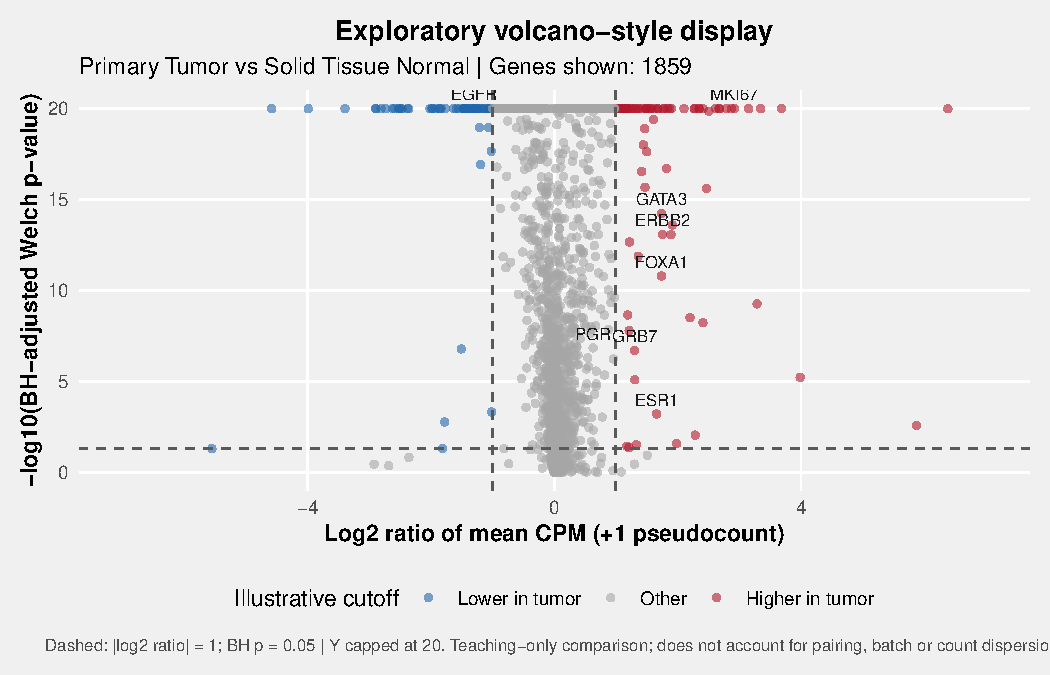
\includegraphics[width=0.85\textwidth]{figures/gene_volcano.pdf}
    \caption{Exploratory volcano plot of gene-expression
    differences between comparison groups.}
    \label{fig:volcano}
\end{figure}

% ============================================================
% TABLES WORKING NO TOUCH
% ============================================================

\clearpage
\section*{Tables}

% Table 1
\begin{table}[H]
\centering
\caption{Primary tumors with a recorded PAM50 subtype
($n = 1{,}099$).}
\label{tab:pam50_distribution}

\small
\begin{tabular}{lrr}
\toprule
Subtype & Samples & Percent (\%) \\
\midrule
Basal  & 197 & 17.9 \\
Her2   & 82  & 7.5 \\
LumA   & 571 & 52.0 \\
LumB   & 209 & 19.0 \\
Normal & 40  & 3.6 \\
\bottomrule
\end{tabular}
\end{table}

% Table 2
\begin{table}[H]

\caption{\label{tab:export-latex-tables}ESR1 and ERBB2 raw-count descriptive statistics.}
\centering
\begin{tabular}[t]{lrrrrrrrr}
\toprule
Gene & N & Missing & Mean & Median & SD & IQR & Min & Max\\
\midrule
ESR1 & 1,231 & 0 & 31,442.2 & 17,561 & 38,261.2 & 40,242.5 & 14 & 270,977\\
ERBB2 & 1,231 & 0 & 46,982.5 & 19,125 & 105,287.5 & 19,287.0 & 205 & 995,067\\
\bottomrule
\end{tabular}
\end{table}


% Table 3
\begin{table}[H]

\caption{\label{tab:export-latex-tables}ESR1 raw-count statistics by PAM50 molecular subtype.}
\centering
\begin{tabular}[t]{lrrrrrrr}
\toprule
Subtype & N & Mean & Median & SD & IQR & Min & Max\\
\midrule
Basal & 197 & 924.5 & 262.0 & 3,589.1 & 620.0 & 14 & 47,589\\
Her2 & 82 & 3,414.2 & 652.5 & 7,745.6 & 2,010.8 & 14 & 40,971\\
LumA & 571 & 43,811.7 & 29,436.0 & 39,799.2 & 43,034.5 & 223 & 270,977\\
LumB & 209 & 53,197.4 & 40,849.0 & 41,119.8 & 46,128.0 & 3,686 & 210,656\\
Normal & 40 & 6,066.0 & 3,922.5 & 7,775.7 & 5,626.5 & 201 & 39,845\\
\bottomrule
\end{tabular}
\end{table}


\clearpage

\FloatBarrier
\clearpage

% ============================================================
% AI DISCLOSURE NO TOUCH
% ============================================================

\section*{AI Disclosure}
AI was used to type in the file names for the figures. The main file before modifications was cleaned by AI from an old manuscript to empty the file, and pre-cook with reporting basic instructions - NO AI USED FOR MANUAL TYPE UP. After template was cooked, this was hand written, and typed with the exception of the file names. 
VIEW GITHUB for documentation chain. 
\newpage

% ============================================================
% REFERENCES IMPORT WORKING NO TOUCH
% ============================================================

\printbibliography[title={References}]
\end{document}
